\section{Introduction}
\index{Probabilistic Risk!PSHA-based}
The classical PSHA-based risk calculator can be used to calculate loss exceedance curves for single \glspl{asset}, calculated site by site, using hazard curves. This calculator thus requires hazard curves as an input, which the engine can calculate using the oq-hazardlib. Currently, this calculator is only capable of computing \gls{groundupLosses}, though \gls{insuredLosses} will be covered in future releases.

\section{Calculation Steps}

\begin{enumerate}

\item By default, the oq-hazardlib computes hazard curves for a set of intensity measure levels that are pre-defined in the configuration file. If the user wishes to use oq-hazardlib to compute the hazard for the risk calculations, then a feature can be used which reads the \gls{vulnerability model} and uses the intensity measure levels (IMLs) defined therein when producing the hazard curve. If instead externally produced hazard curves are used, the user needs to ensure that the IMLs in the hazard curves cover the full range required by the \glspl{vulnerability function}. 

\item To use this calculator, the hazard curves need first to be converted into probability mass functions (e.g. probability of occurrence of a discrete set of intensity measure levels). To do so, the engine starts by reading the intensity measure levels from the discrete \glspl{vulnerability function}, and computes the central value between consecutive levels. Two consecutive values define the boundaries of the interval for each intensity measure level and by relating these limits with the hazard curve, the engine computes the corresponding probabilities of exceedance. Figure \ref{fig:ProbOccurrence} contains a discrete \gls{vulnerability function} (bottom figure) and a hazard curve (top figure) in which the definition of the interval for a given intensity measure level and associated estimation of the probabilities of exceedance of each limit are illustrated. 

\begin{figure}[ht]
\centering
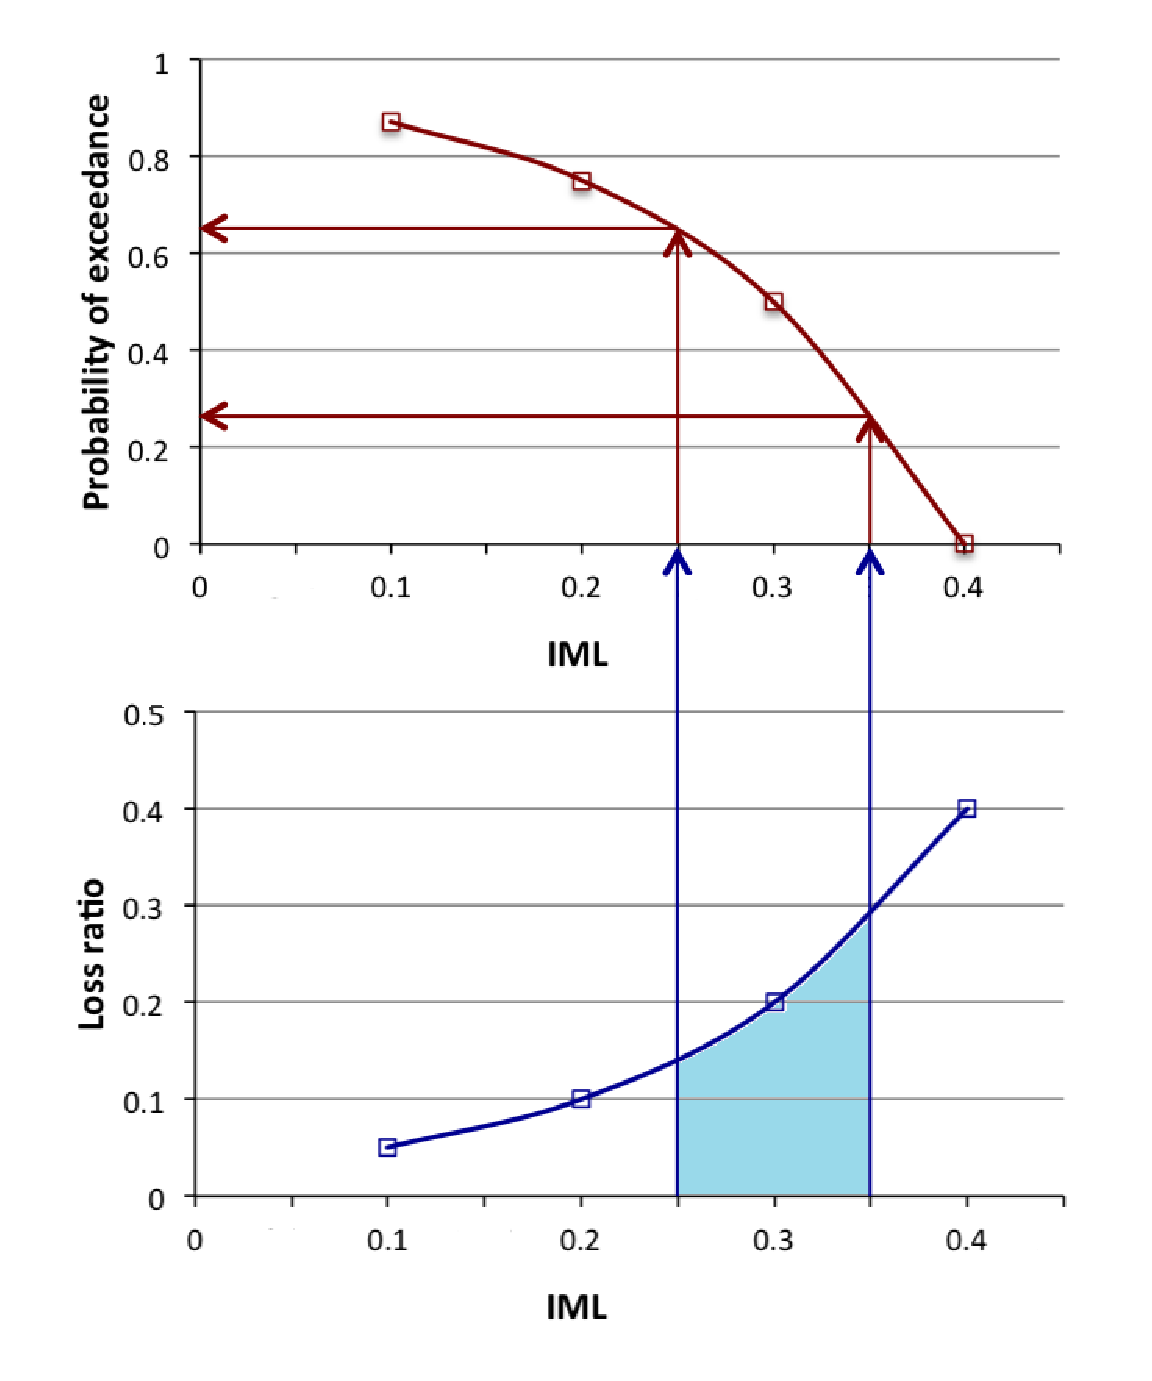
\includegraphics[width=6.5cm,height=7cm]{./figures/risk/ProbOccurrence.eps}
\caption{Workflow to estimate the probabilities of exceedance of the boundaries of each intensity measure level.}
\label{fig:ProbOccurrence}
\end{figure}

\item The probability of occurrence of the intensity measure levels that fall within each interval can be derived by subtracting the probabilities of exceedance of the lower and upper limits, as described by the following formula:

\begin{equation}
PO= PE[lower bound]-PE[upper bound]
\end{equation}

\item The discrete \glspl{vulnerability function} for each \gls{asset} are converted into loss ratio exceedance matrices (e.g. matrices which describe the probability of exceedance of each loss ratio for a discrete set of intensity measure levels). These matrices have a number of columns equal to the number of intensity measure levels defined on the \gls{vulnerability function} and a number of rows that can go from the number of loss ratios defined by the discrete function, up to any multiple of this number. In order to properly incorporate the probabilistic distribution of loss ratios per intensity measure level, the probabilities of exceedance should be computed not just for the loss ratios defined on the \gls{vulnerability function}, but also for many intermediate values between consecutive loss ratios. Following a number of sensitivity analyses, it appears that 5 intermediate values between consecutive loss ratios is a reasonable value, however, this is a parameter that can be adjusted by the user. Figure \ref{fig:LREM} contains an example of a discrete \gls{vulnerability function} and the respective loss ratio exceedance matrix (in light grey).

\begin{figure}[htb]
\centering
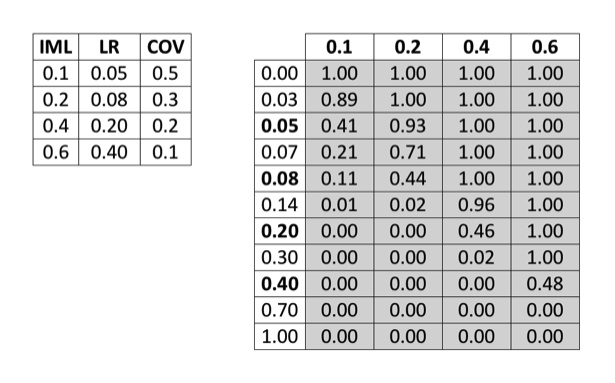
\includegraphics[width=9cm,height=5.5cm]{./figures/risk/LREM.eps}
\caption{Example of a discrete vulnerability function and respective loss ratio exceedance matrix.}
\label{fig:LREM}
\end{figure}

Note that for this example only one intermediate value was considered between consecutive loss ratios and in order to consider the whole distribution of the loss ratios, the matrix was computed considering a minimum and maximum loss ratio of 0 and 1 respectively.

\item Finally, each column of the aforementioned matrix is multiplied by the probability of occurrence of the respective intensity measure level (extracted from the hazard curves) to produce a conditional loss ratio exceedance matrix.  Then, for each loss ratio the probabilities of exceedance are summed, leading to a loss ratio exceedance curve, whose set of loss ratios can be multiplied by the value of the \gls{asset} given by the \gls{exposure model} to obtain an absolute loss exceedance curve.

\end{enumerate}

\section{Calculator Output}
The output of this calculator comprises loss exceedance curves and loss maps. Loss exceedance curves are represented by a list of losses and respective probabilities of exceedance. Furthermore, each curve is associated with a pair of coordinates, an end branch label (that allows the curve to be connected to the set of specifications used in the calculations) and an asset ID (that permits tracking of the asset that each loss curve was computed for). Loss maps for a given probability of exceedance in a given time span can be produced, as well as maps of mean loss within a given time span, similarly to what has been described in the Probabilistic Event-based risk calculator.
